\documentclass[singlecolumn,11pt]{pnas-new}
% Use the lineno option to display guide line numbers if required.
% Note that the use of elements such as single-column equations
% may affect the guide line number alignment. 

%Many authors find it useful to organize their manuscripts with the following order of sections;  Title, Author Affiliation, Keywords, Abstract, Significance Statement, Results, Discussion, Materials and methods, Acknowledgments, and References. Other orders and headings are permitted.

\usepackage[super]{nth} %adds superscripts for things like 20th

\templatetype{pnasresearcharticle} % Choose template 
% {pnasresearcharticle} = Template for a two-column research article
% {pnasmathematics} = Template for a one-column mathematics article
% {pnasinvited} = Template for a PNAS invited submission

\title{Supplementary Information for The Changing Character of Banded Rainfall in China, 1951-2007}

\author[a,1]{Jesse Day}
\author[a]{Inez Fung} 
\author[b]{Weihan Liu}

\affil[a]{Department of Earth and Planetary Science, University of California Berkeley, 94103}
\affil[b]{College of Letters and Sciences, University of California Berkeley, 94103}

% Please give the surname of the lead author for the running footer
\leadauthor{Day} 

\begin{document}

\maketitle

\dates{This manuscript was compiled on \today}

\makeatletter 
\renewcommand{\thefigure}{S\@arabic\c@figure}
\makeatother


\section*{Supporting Information (SI)}

\subsection{RDA Algorithm}
Key aspects of the Rainband Detectional Algorithm (RDA) are exhibited in Supplementary Figures~\ref{fig:algo_1}-\ref{fig:algo_4}.

\subsection{Alternative Metrics of China Rainfall}

Since the RDA method is complex, we must justify its use by proving that it supplies information about China rainfall beyond what simpler metrics can provide. We tested the following suite of daily rainfall metrics:

\begin{itemize}

	\item $M_1$ - Latitude of maximum rainfall;
	
	\item $M_2$ - Intensity-weighted centroid of daily rainfall latitude;
	
	\item $M_3$ - Intensity of maximum rainfall over China (100-123$^{\circ}$E and 20-40$^{\circ}$N);
	
	\item $M_4$ - Area-averaged intensity of China rainfall; 
	
	\item $M_5$ - Area-averaged intensity of North China rainfall (107.5-125$^{\circ}$E and 37-42$^{\circ}$N); 
	
	\item $M_6$ - Area-averaged intensity of South China rainfall (107.5-122.5$^{\circ}$E and 27-33$^{\circ}$N); 
	
	\item $M_7$ - \% of days where $M_5$ exceeds 1 mm day$^{-1}$ (\textit{frequency} of North China rainfall);
	
	\item $M_8$ - \% of days where $M_6$ exceeds 1 mm day$^{-1}$ (\textit{frequency} of South China rainfall).
	
\end{itemize}

 The definitions of the North China and South China regions are the same as in \cite{Yu2010}. Figures~\ref{fig:alternative_metrics} and \ref{fig:alternative_metrics_2} compare annual climatologies for 1980-2007 versus 1951-2007 and 1994-2007 versus 1980-1993 respectively. In general, the changes in these metrics are fewer and less discernible than those revealed by the use of RDA.
 
 \subsection{Temporal Autocorrelation}

	Fronts and rainbands tend to persist for several days. Therefore, rainfall amounts and front attributes on successive days are not fully independent observations, which reduces the effective number of degrees of freedom of these time series. This temporal autocorrelation must be accounted for in calculations of statistical significance such as estimating the $p$-value of a change in rainband frequency between two time periods. In this particular case, we use the analytic formula for a Bernoulli process (applicable for any time series where observations are binary) with effective number of degrees of freedom $n=\frac{N}{\tau}$ for number of days $N$ and decorrelation time $\tau$ given by

\begin{equation*}
\tau=1+2\sum_{k=1}^m \rho(k)
\end{equation*}

	where $\rho(k)$ is the autocorrelation function of rainband existence with lag $k$ \citep{VonStorch1999}. We calculate $\tau$ using a maximum lag of $m=10$ days. The yearly mean decorrelation timescale of rainband frequency is found to be $\tau = 1.81$ after removing the seasonal cycle. This value is used to calculate significance of changes in Figure 3b. The standard deviation and $p$-values of rainband frequency shown in Figure 4 use seasonal values of $\tau$ shown in \cite{Day2016}. $\tau$ is also used to select block length for moving blocks bootstrap tests, as described below.
 
\subsection{Significance of Changes}

\subsubsection{Bootstrapping with and without Replacement}

	Observations of rainband latitude and intensity during a given time period obey unknown distributions. Therefore, we require non-parametric tests to estimate the standard deviation of their mean and the significance of changes in mean. We employ bootstrapping with and without replacement (the latter also known as a permutation test), well-established techniques that estimate quantities of interest by constructing synthetic distributions with random sampling of original data \citep{Good2005}. We calculate the significance of changes in mean rainband latitude and intensity between 1951-1979 and 1980-2007, and also repeat our methodology for 1980-1993 versus 1994-2007 (Figure 4).

\subsubsection{Moving Blocks Bootstrap}	
	
	The bootstrap must be adapted for time series featuring temporal autocorrelation. In such time series, a single anomalous weather event will persist over several days, and a bootstrap method will tend to exaggerate the significance of differences between the two original distributions. To avoid this scenario, we use a \textit{moving blocks bootstrap} test, described for instance in \citet{Singh2014}. This technique is identical to bootstrapping with replacement except that samples are drawn in continuous blocks of length $n$ that preserve the time structure of the original data set. Block length is chosen based on decorrelation time scale $\tau$. The autocorrelation of daily rainfall in China is approximately $\tau =2-3$ days, and therefore the significance estimates in Figure 5a and b use a moving blocks bootstrap with block length of 2 days and 2000 iterations. In general, a choice of block lengths between 2 and 5 days leads to similar results. Our MATLAB code for the permutation test and the moving blocks bootstrap is included in the appendix.
	
\subsection{Significance of Changes in Distribution}

	A moving blocks bootstrap cannot be used for time series with gaps. However, using a permutation test to estimate the significance of changes in the mean of latitude and intensity may overestimate their significance. Therefore, we verify results by also implementing a Kolmogorov-Smirnov (K-S) and Anderson-Darling (A-D) tests, each of which estimates the probability that two samples were drawn from the same distribution. Both the K-S and A-D tests define a test statistic based on the largest difference between the observed probability distribution of two samples. Similar to a $t$-test, the value of this test statistic can be translated into a $p$-value. We first define the \textit{empirical distribution function} $F_1(x)$ and $F_2(x)$ of each sample. All $n$ observations in each sample are ordered as $\left\{X_1 < ... < X_n\right\}$, after which $F(x)$ is calculated as follows:

\begin{align}
	F(x) =& \frac{1}{n}\sum_{i=1}^n I_{[-\infty,x]} (X_i) \\
	I_{[-\infty,x]} =& 
	\begin{cases}
   		 1 & \text{if } X_i \leq x\\
    		0 & \text{otherwise} \\
    	\end{cases}
\end{align}

 The K-S test statistic $D$ is then defined as the maximal distance between the two empirical distribution functions:

\begin{equation}
	D=\max_{all\ x} |F_{1}(x)-F_{2}(x)|
\end{equation}

$D$ can then be inverted to derive a $p$-value. The Anderson-Darling (A-D) test statistic $A^2$ resembles $D$, but is formulated to be more sensitive to the tails of the distribution:

\begin{equation}
	A^2 = -n-S \,,
	\mathrm{where}
\end{equation}

\begin{equation}
	S=\sum_{i=1}^n \frac{2i-1}{n}\left[\ln(F(X_i)) + \ln\left(1-F(X_{n+1-i})\right)\right].
\end{equation}

	$A^2$ can likewise be translated into a $p$-value. The K-S and A-D tests cannot be used if values are repeated within samples, because $D$ and $A^2$ are then undefined. We solve this problem by using bootstrap versions of these tests. Bootstrap K-S and A-D tests were performed as tests in R with 10,000 iterations. The significance of changes in the distribution of rainband latitude and intensity were previously presented in \cite{Day2016}. Both tests produce fairly similar results.
	
\clearpage

%%EXPLANATORY FIGURES SHOWING ALGORITHM FUNCTIONALITY

%%FIGURE S1 - displaying continuous maximum criterion required to attempt rainband fit
\begin{figure}[htbp]
\centering
\noindent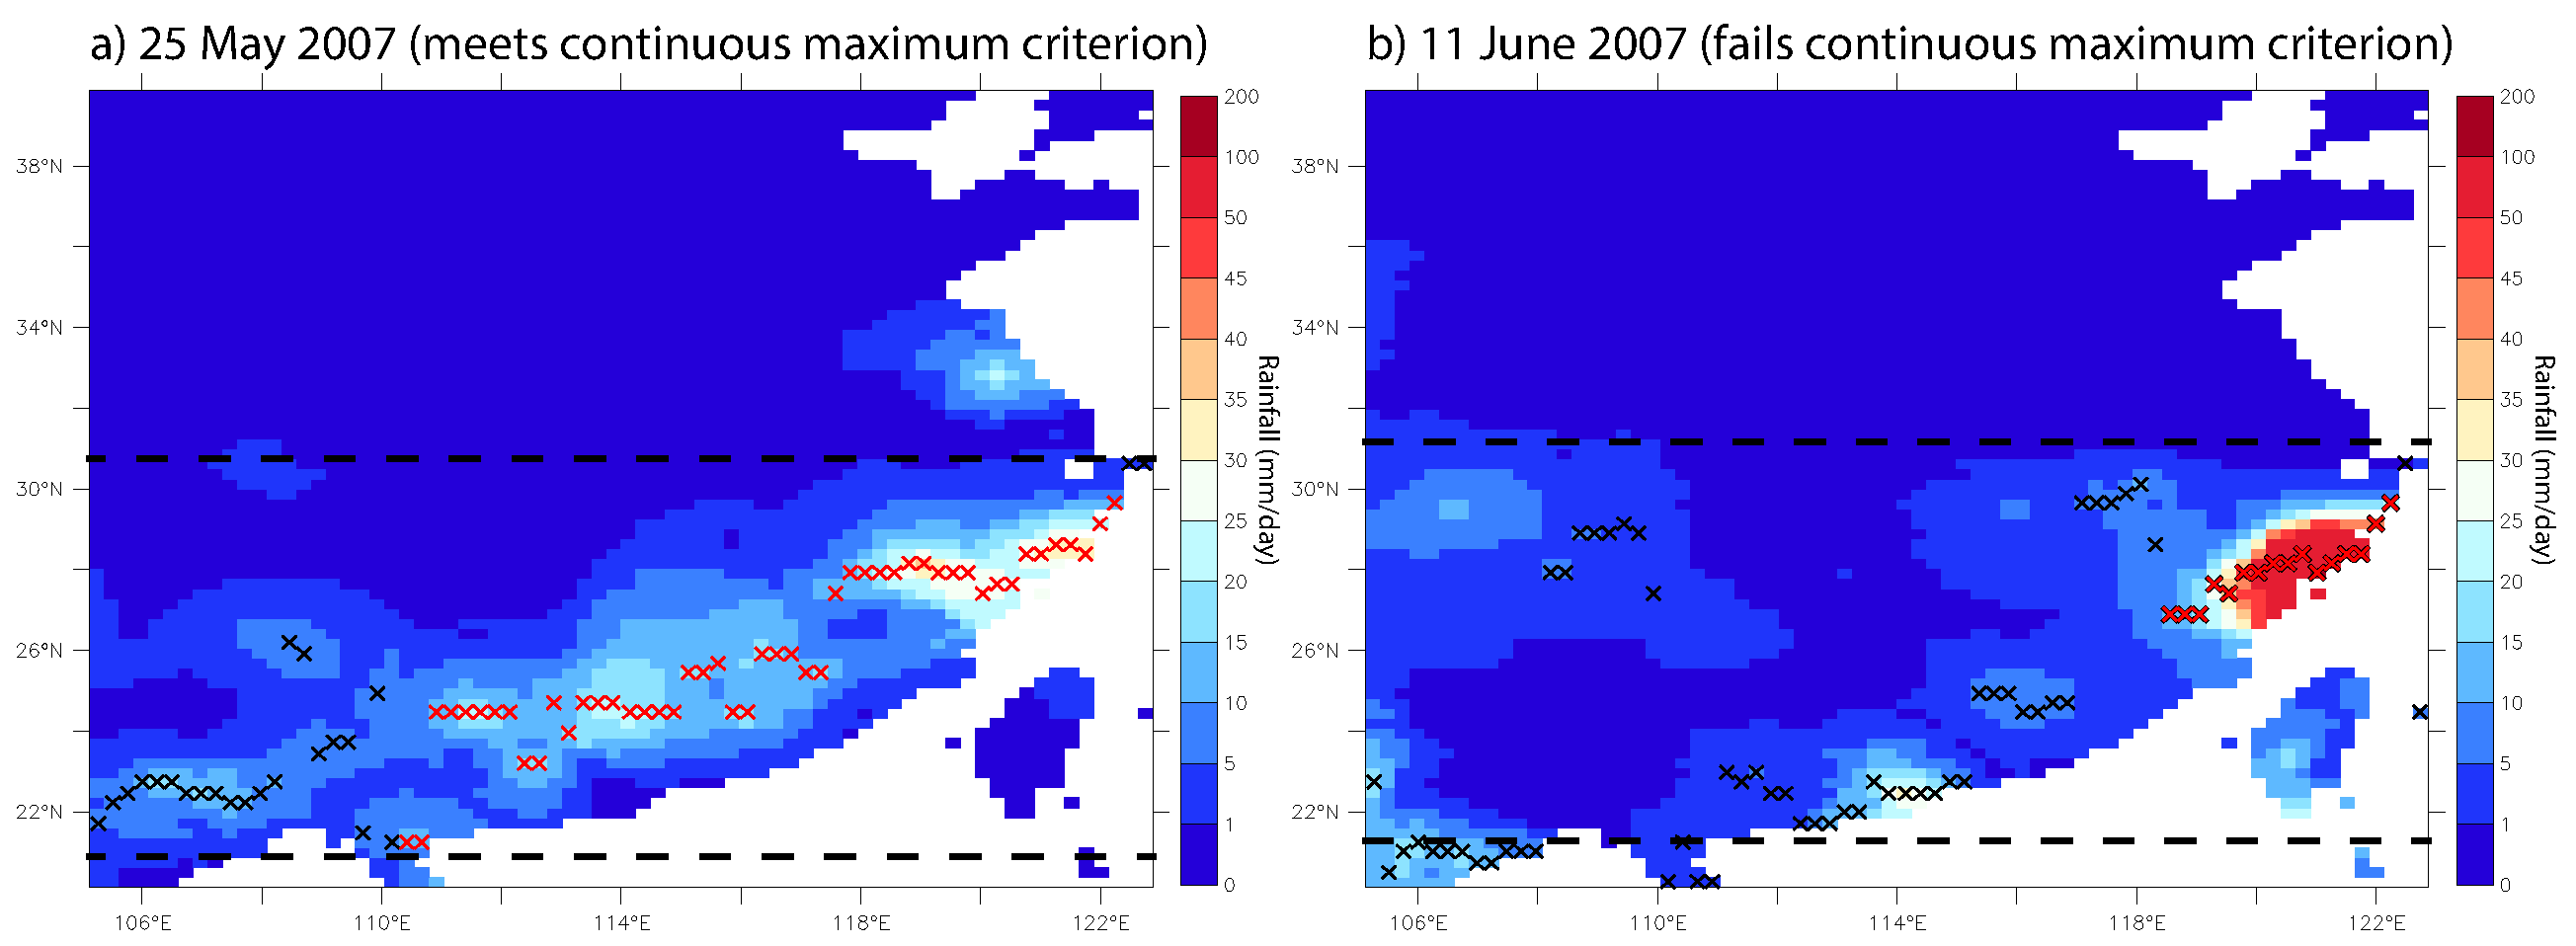
\includegraphics[width=39pc]{Figures/S1}
\caption{On each day, RDA first checks whether a continuous band of precipitation maxima exceeding 10 mm day$^{-1}$ exists that spans over 5 degrees of longitude. If so, a rainband fit is attempted. In panels a and b, the latitude of maximum precipitation at each longitude is marked with a black X. The longest continuous chain of maxima exceeding 10 mm day$^{-1}$ is marked in red. a) 25 May 2007 - the continuous maximum criterion is met and a fit is attempted.  b) 11 June 2007 - although there is abundant rainfall in some locations, no band is visible and the continuous maximum criterion is failed. No fit is attempted.}
\label{fig:algo_1}
\end{figure}

%%FIGURE S2 - How the convergent fit algorithm works.
\begin{figure}[htbp]
\centering
\noindent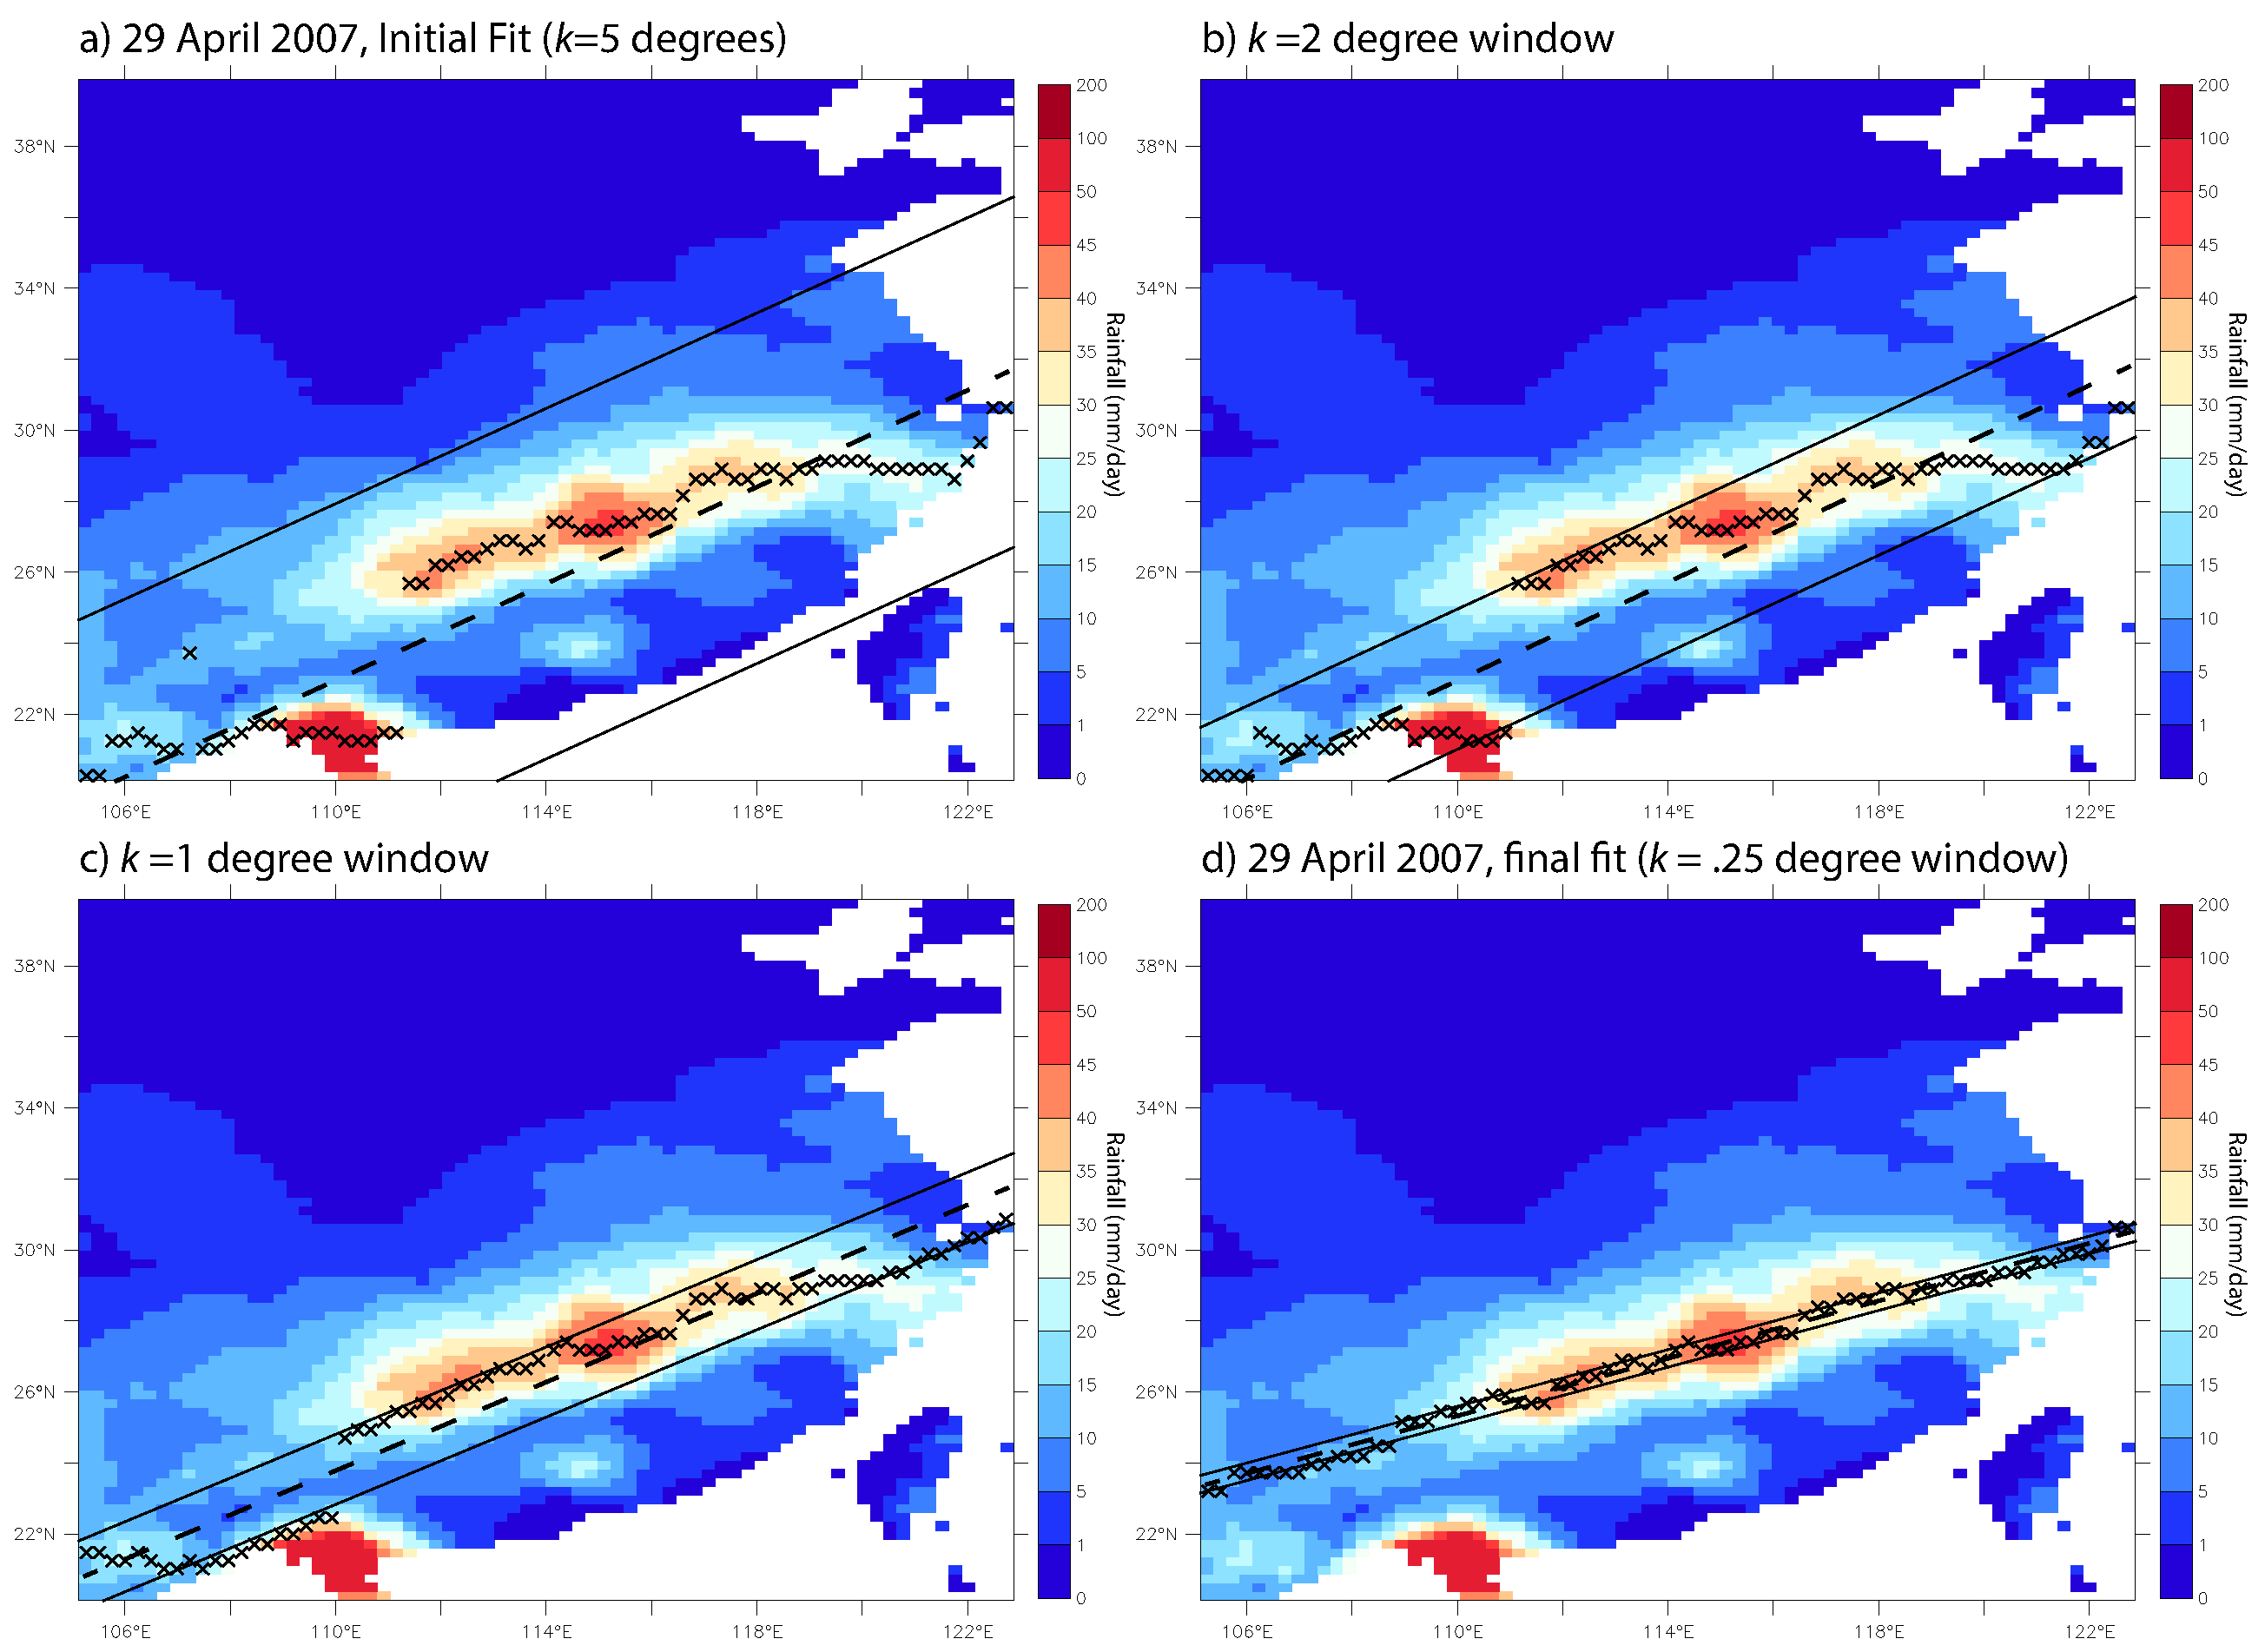
\includegraphics[width=39pc]{Figures/S2}
\caption{Display of the functionality of the recursive convergent fit. Dashed line shows estimated rainband position before each iteration and the solid lines indicate the window within we search for maxima. On 29 April 2007, a strong maximum in southernmost China skews our initial rainband fit (a), but the algorithm eventually converges on its true position via tighter windowing (d).}
\label{fig:algo_2}
\end{figure}

\clearpage

%%FIGURE S3 - Quality Control algorithm used to determine inclusion in statistics
\begin{figure}[htbp]
\centering
\noindent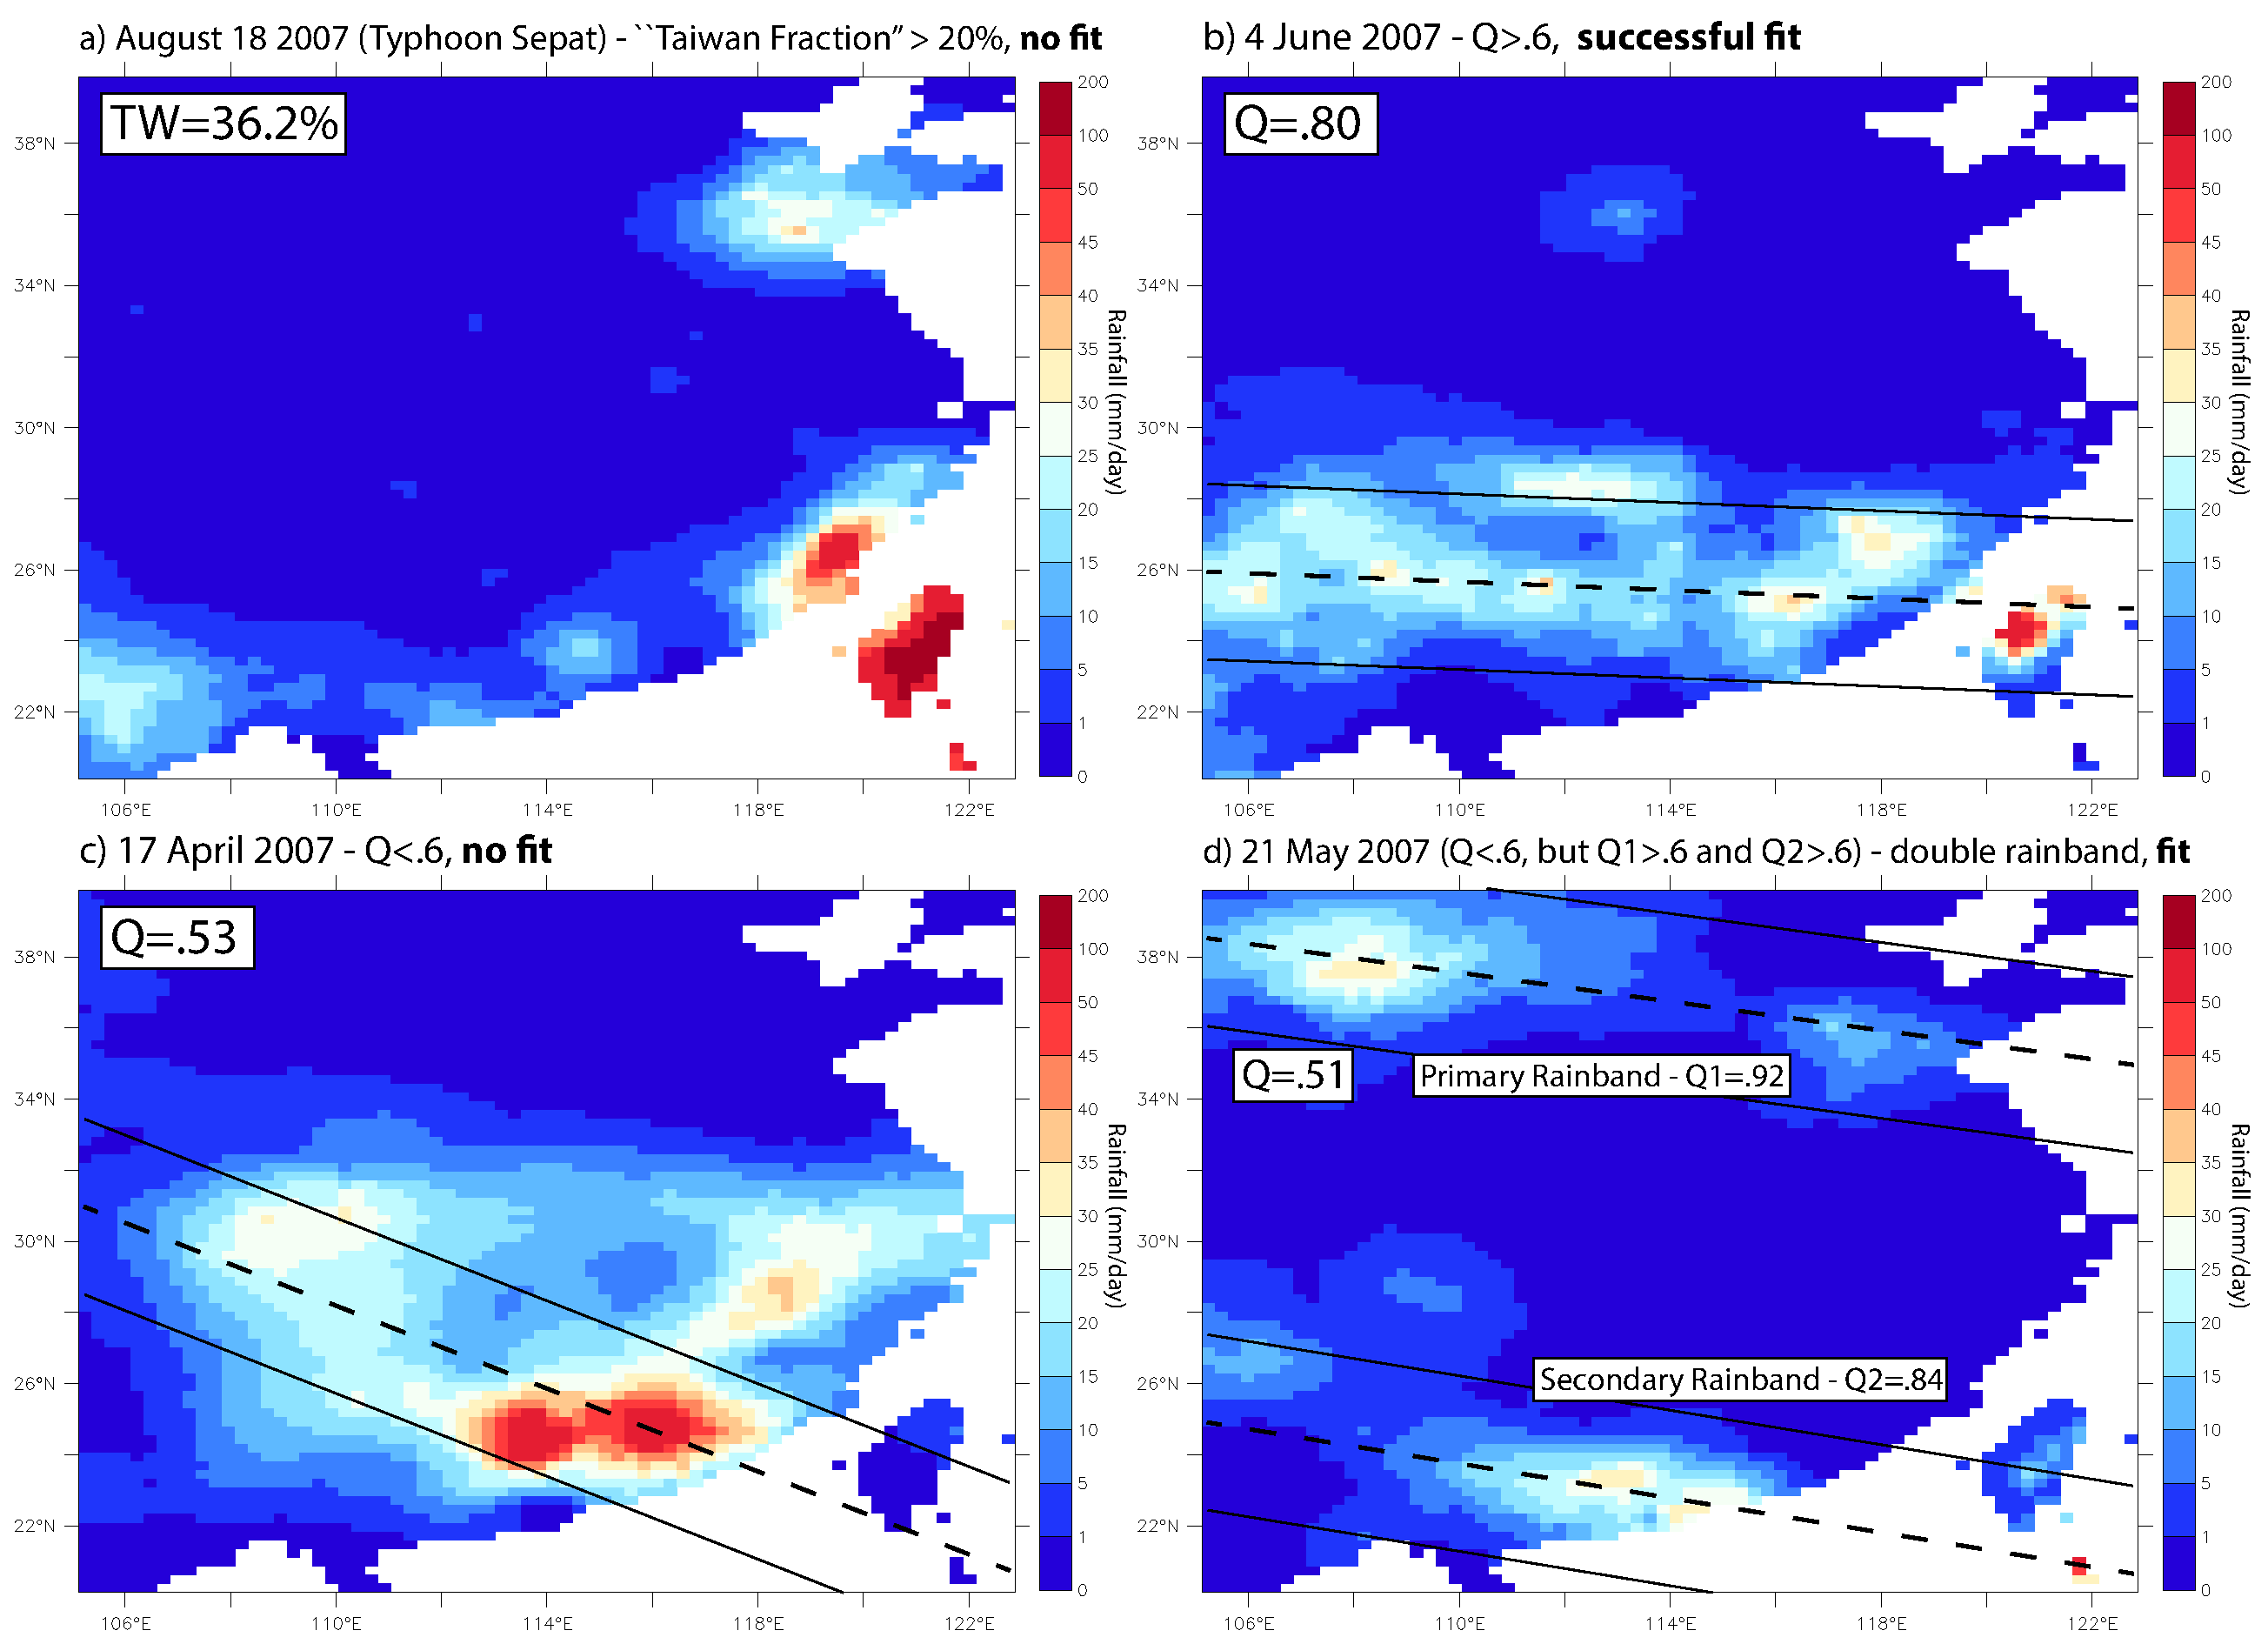
\includegraphics[width=39pc]{Figures/S4}
\caption{A quality control algorithm is used to exclude poor fits. a) 18 August 2007 - Days with a high Taiwan fraction (here, corresponding to the passage of Typhoon Sepat) are excluded from our statistics. b) June 4 2007 - A high-quality fit is achieved. c) 17 April 2007 - Although a tentative fit is obtained, it explains the distribution of rainfall poorly and is therefore unsuccessful. d) 21 May 2007 (same day as Figure~\ref{fig:algo_4}) - An initial fit appears to be of poor quality ($Q<.6$). However, after finding a secondary rainband, we determine that conditional quality scores $Q_1$ and $Q_2$ are sufficiently high, and the double rainband fit is successful.}
\label{fig:algo_3}
\end{figure}

%%FIGURE S4 - Procedure for finding double rainbands
\begin{figure}[htbp]
\centering
\noindent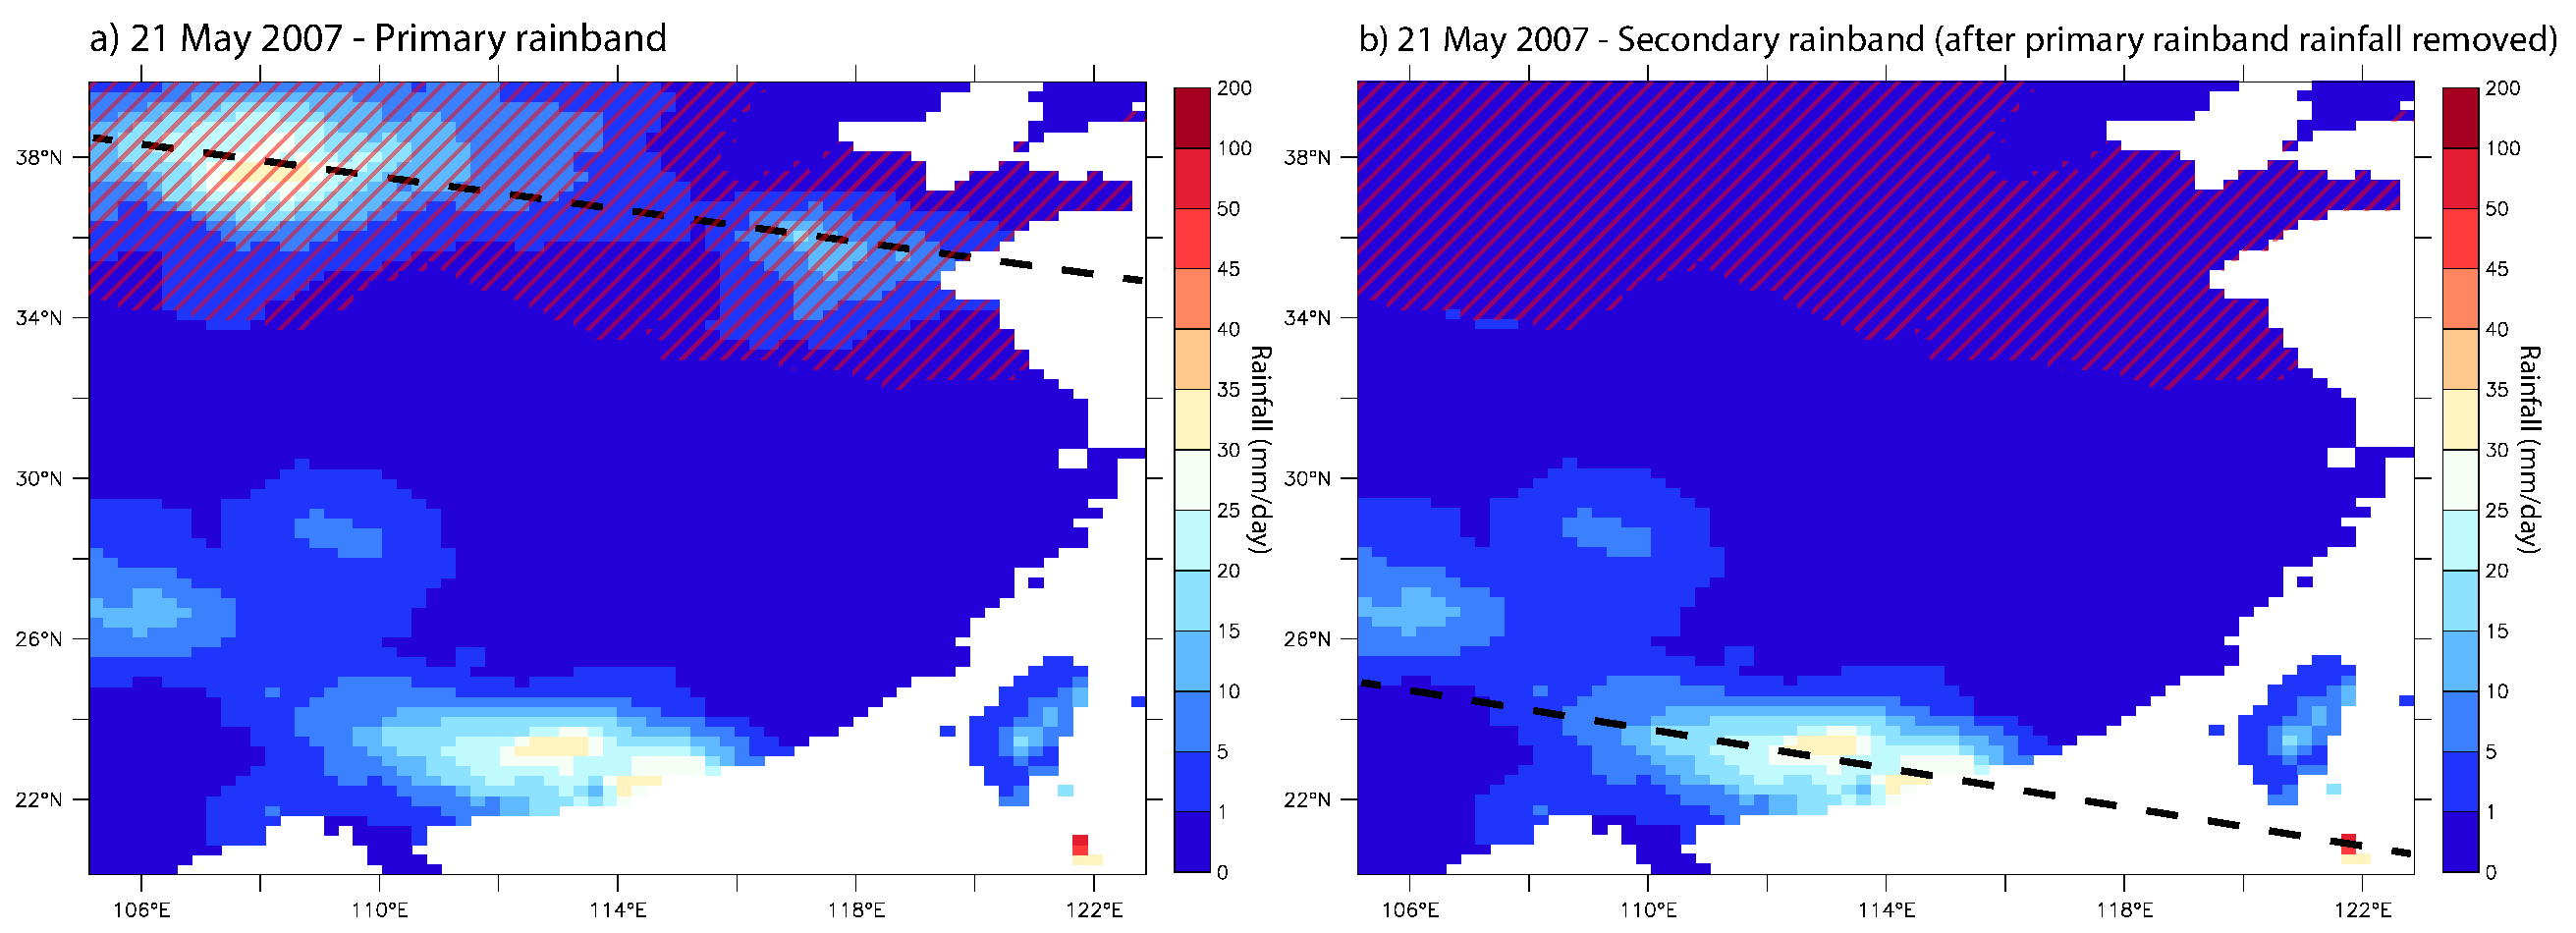
\includegraphics[width=39pc]{Figures/S3}
\caption{a) The first pass of the recursive fit algorithm converges on the strongest rainband, around 37$^{\circ}$N (defined as the ``primary rainband''). The \textit{banded rainfall} associated with the primary band is shaded with red hatchmarks. b) All banded rainfall from the primary band is removed, and we check for the presence of another rainband (a ``secondary rainband''), again using the continuous maximum criterion. When this criterion is satisfied, we find the secondary rainband's position with the recursive fit algorithm.}
\label{fig:algo_4}
\end{figure}

%%FIGURE S5 Decadal mean of banded_frac_climo in different rainfall types during different time periods
\begin{figure}[htb]
\centering
\noindent
\includegraphics[width=38pc]{Figures/banded_frac_climo}
\caption{Climatology of the fraction of all rainfall that falls as banded rainfall for full year, Spring Rains (days 81-120), Pre-Meiyu (days 121-160), Meiyu (days 161-200), Post-Meiyu (days 201-273) and Fall Rains (days 274-320). \textit{Banded} rainfall consists of all rainfall falling within 4$^{\circ}$ of a rainband axis and rainfall at any other adjacent point exceeding 10 mm day$^{-1}$. \textit{Local} rainfall includes all rainfall not meeting these criteria. Note that color bar switches from .5 to 1 mm day$^{-1}$ increment past 5 mm day$^{-1}$.}
\label{fig:banded_frac_climo}
\end{figure}

%%FIGURE S6 - Climatology of banded and local rainfall + area average
\begin{figure}[htbp]
\centering
\noindent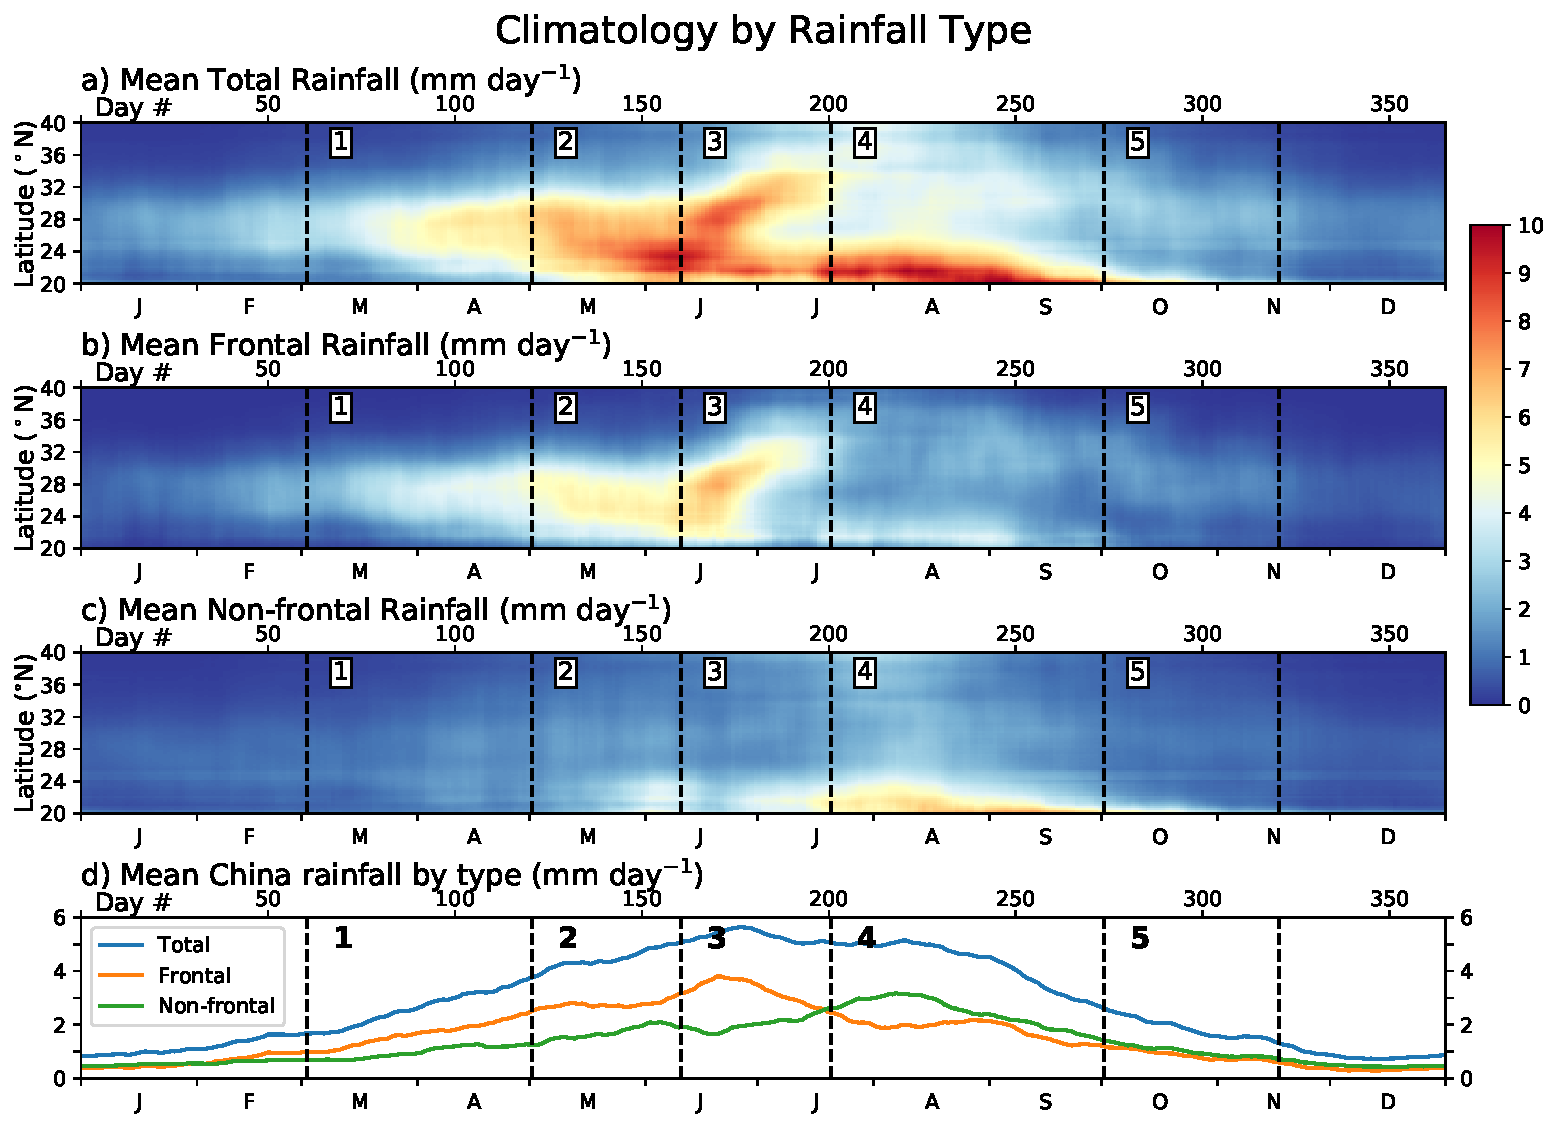
\includegraphics[width=39pc]{Figures/hov_types_climo}
\caption{a) The first pass of the recursive fit algorithm converges on the strongest rainband, around 37$^{\circ}$N (defined as the ``primary rainband''). The \textit{banded rainfall} associated with the primary band is shaded with red hatchmarks. b) All banded rainfall from the primary band is removed, and we check for the presence of another rainband (a ``secondary rainband''), again using the continuous maximum criterion. When this criterion is satisfied, we find the secondary rainband's position with the recursive fit algorithm.}
\label{fig:type_hov}
\end{figure}

%%FIGURE S7 Comparison of alternative metrics of China rainfall, 1980-2007 versus 1951-1979
\begin{figure}[htb]
\centering
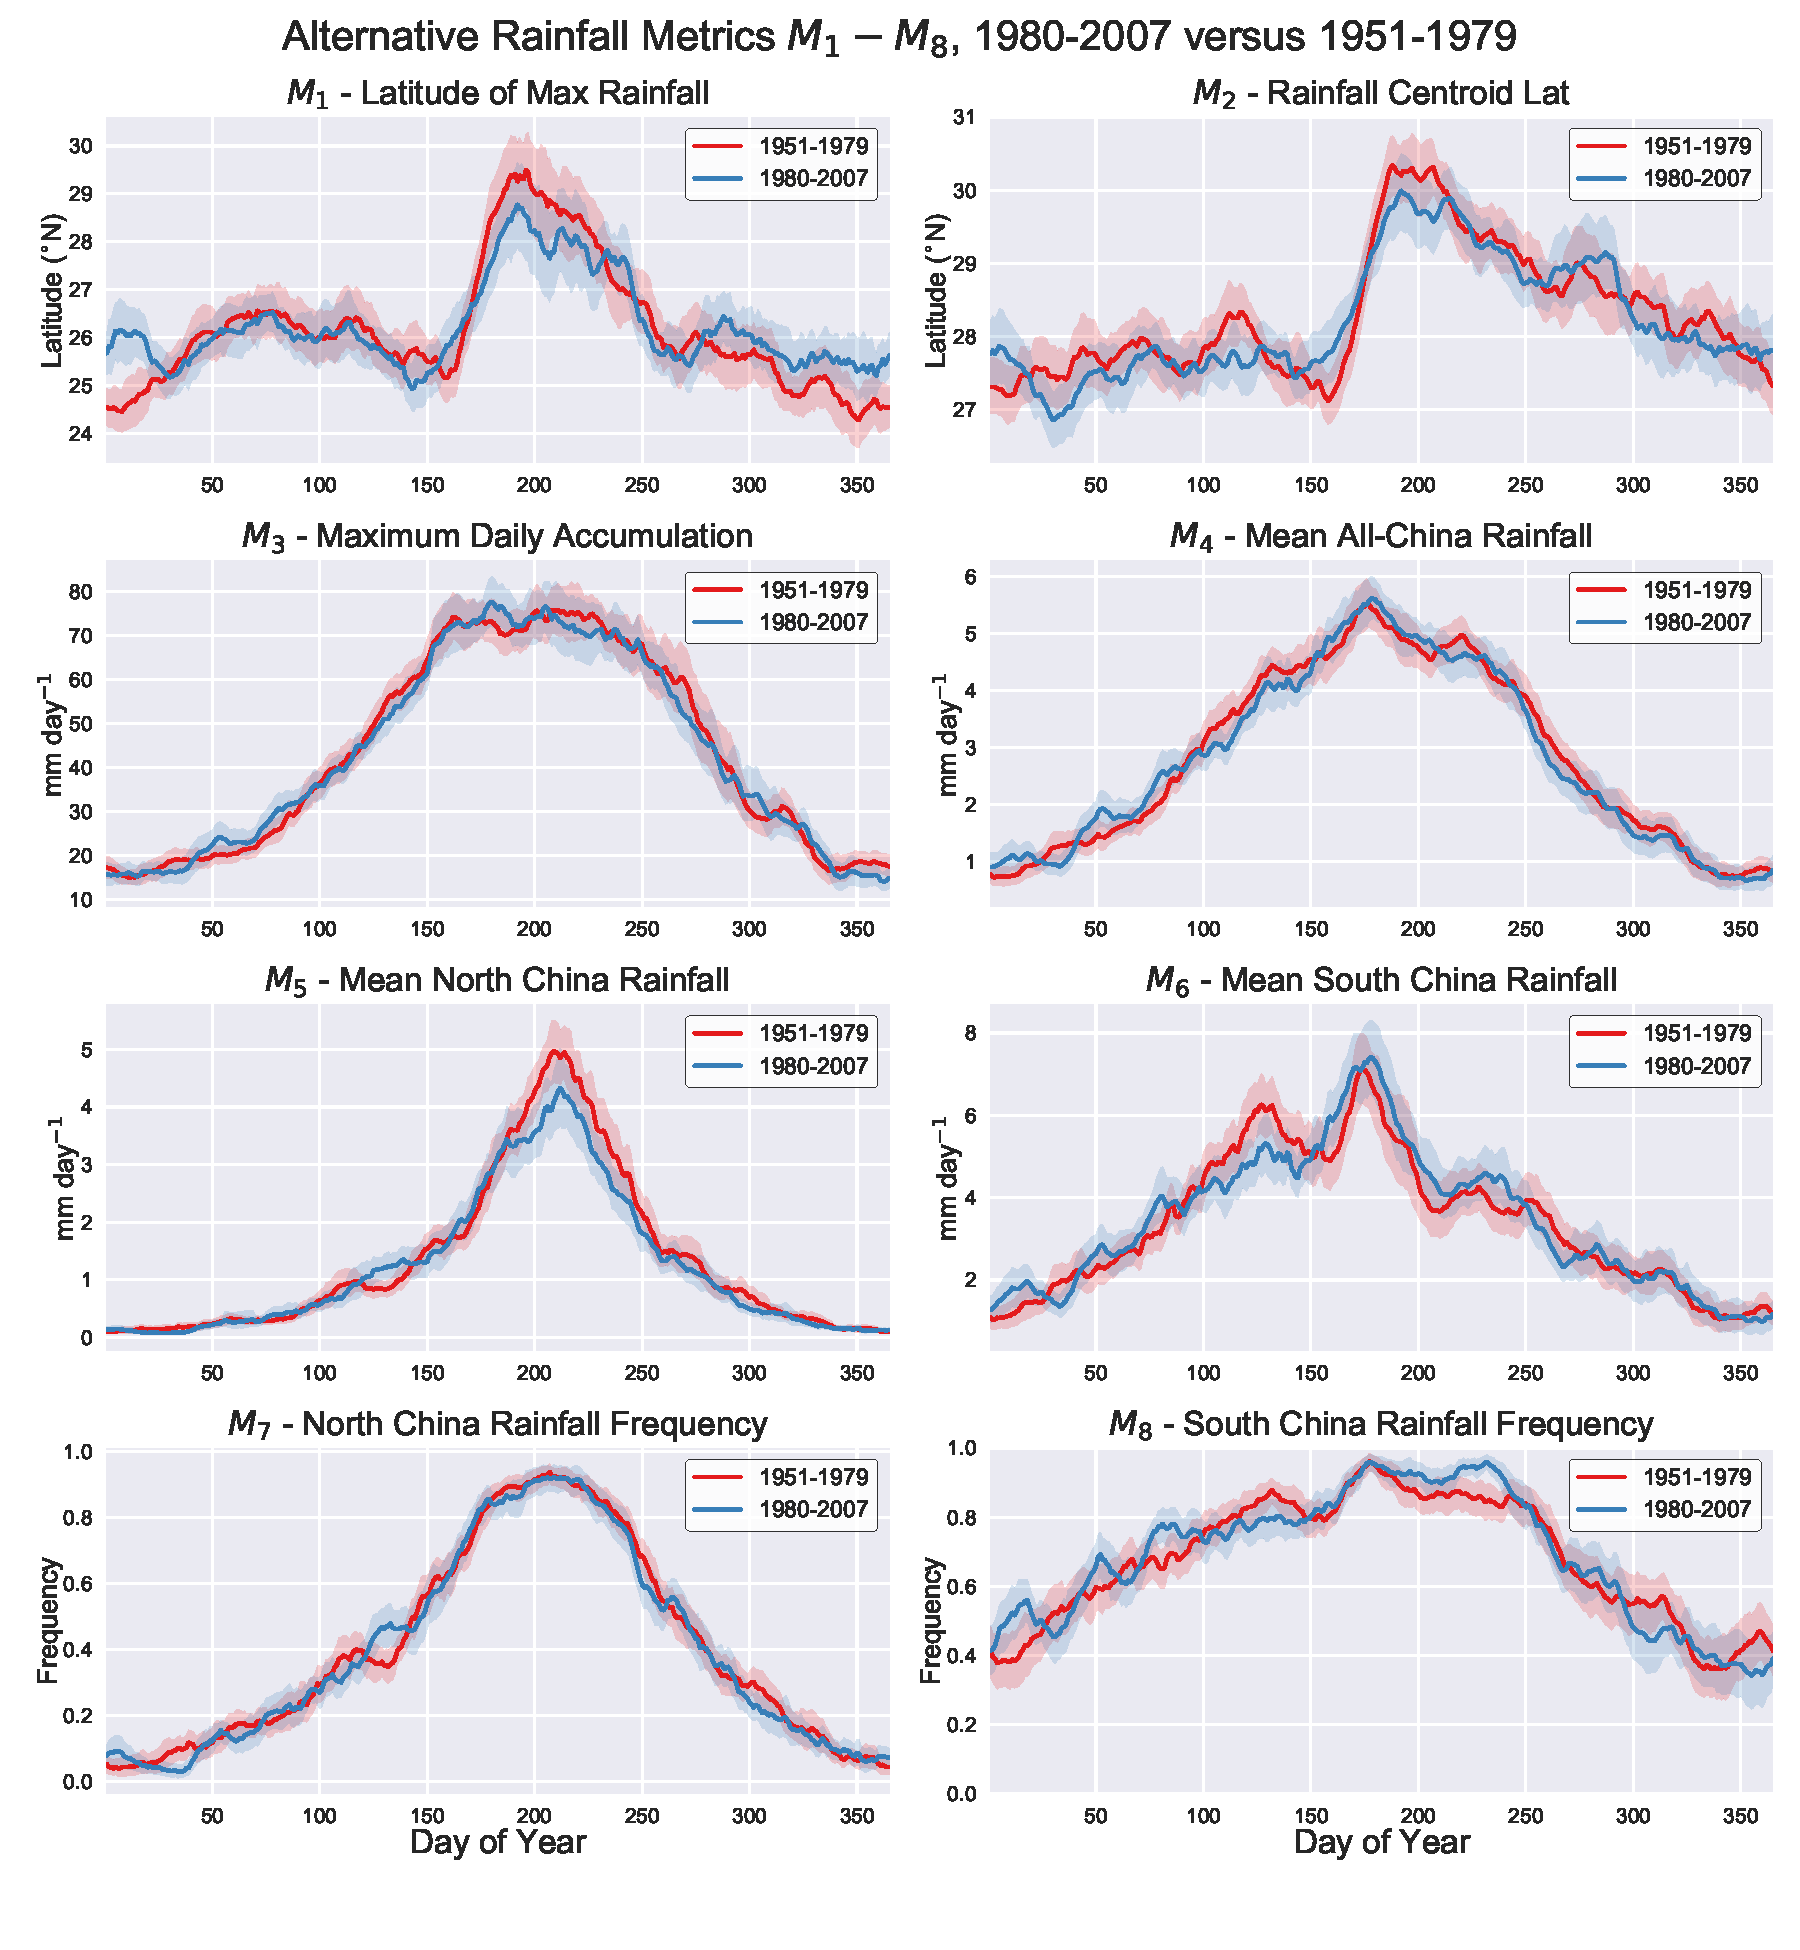
\includegraphics[width=36pc]{Figures/alternative_metrics_8007_5179}
\caption{Climatology of alternative metrics of China rainfall $M_1-M_8$ for time periods 1951-1979 and 1980-2007. China region is defined as 105-123$^{\circ}$E and 20-40$^{\circ}$N, North China as 107.5-125$^{\circ}$E and 37-42$^{\circ}$N and South China as 107.5-122.5$^{\circ}$E and 27-33$^{\circ}$N.}
\label{fig:alternative_metrics}
\end{figure}

%%FIGURE S8 Comparison of alternative metrics of China rainfall, 1994-2007 versus 1980-1993
\begin{figure}[htb]
\centering
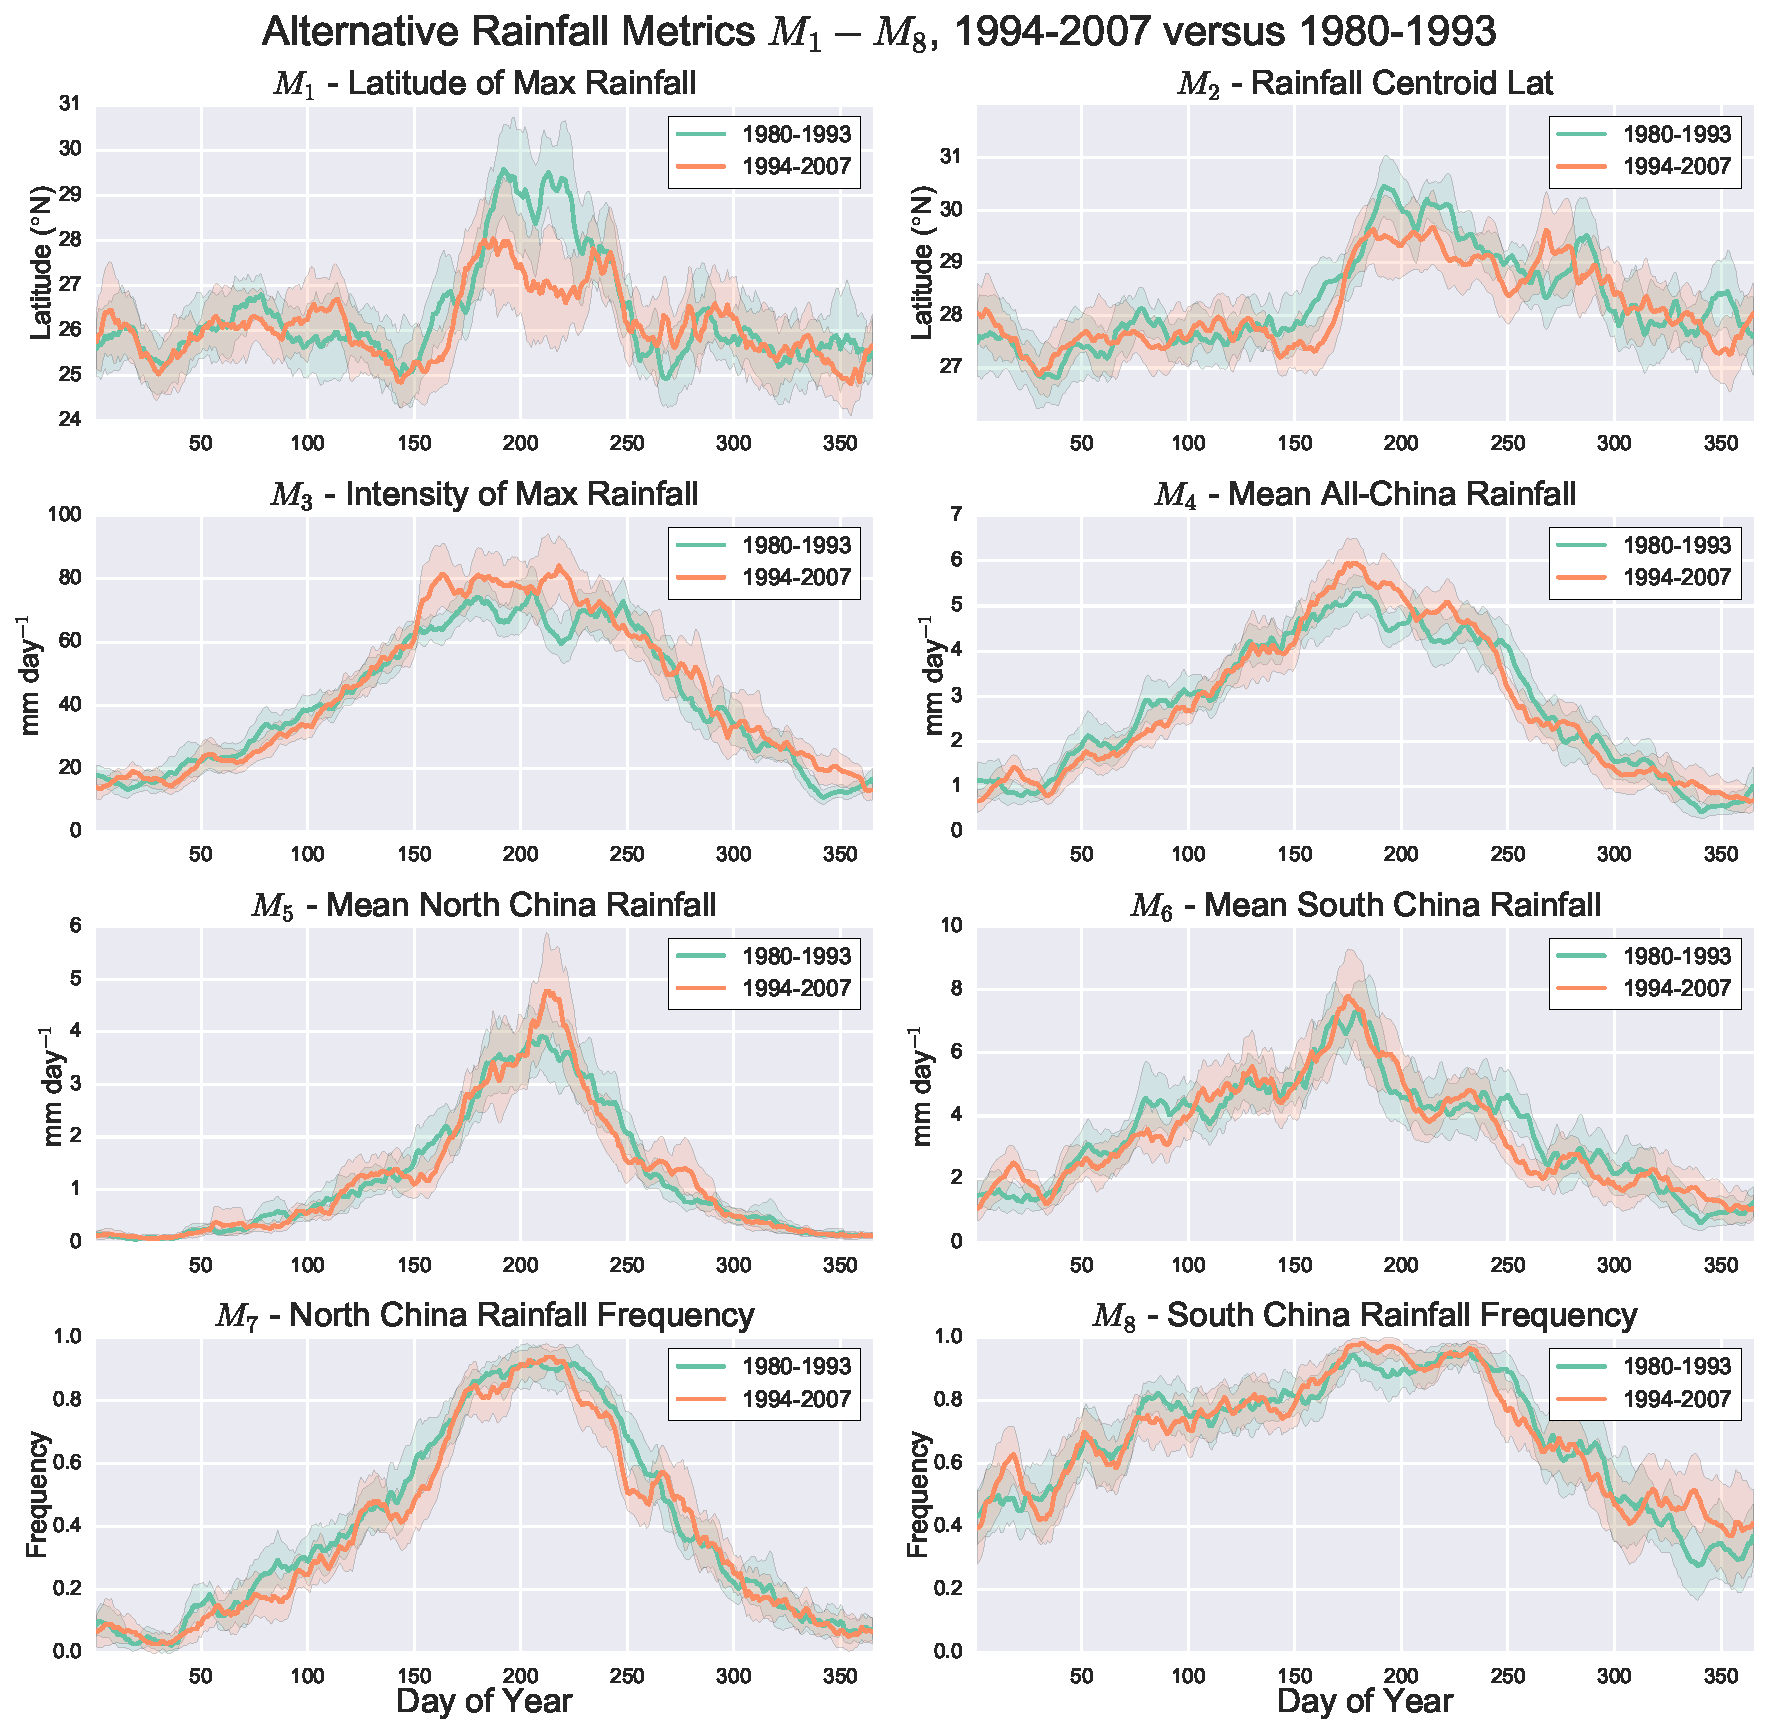
\includegraphics[width=36pc]{Figures/alternative_metrics_9407_8093}
\caption{Climatology of alternative metrics of China rainfall $M_1-M_8$ for time periods 1980-1993 and 1994-2007. China region is defined as 105-123$^{\circ}$E and 20-40$^{\circ}$N, North China as 107.5-125$^{\circ}$E and 37-42$^{\circ}$N and South China as 107.5-122.5$^{\circ}$E and 27-33$^{\circ}$N.}
\label{fig:alternative_metrics_2}
\end{figure}

%%FIGURE S9 - the South Flood-North Drought shown in a single figure.
\begin{figure}
\centering
\noindent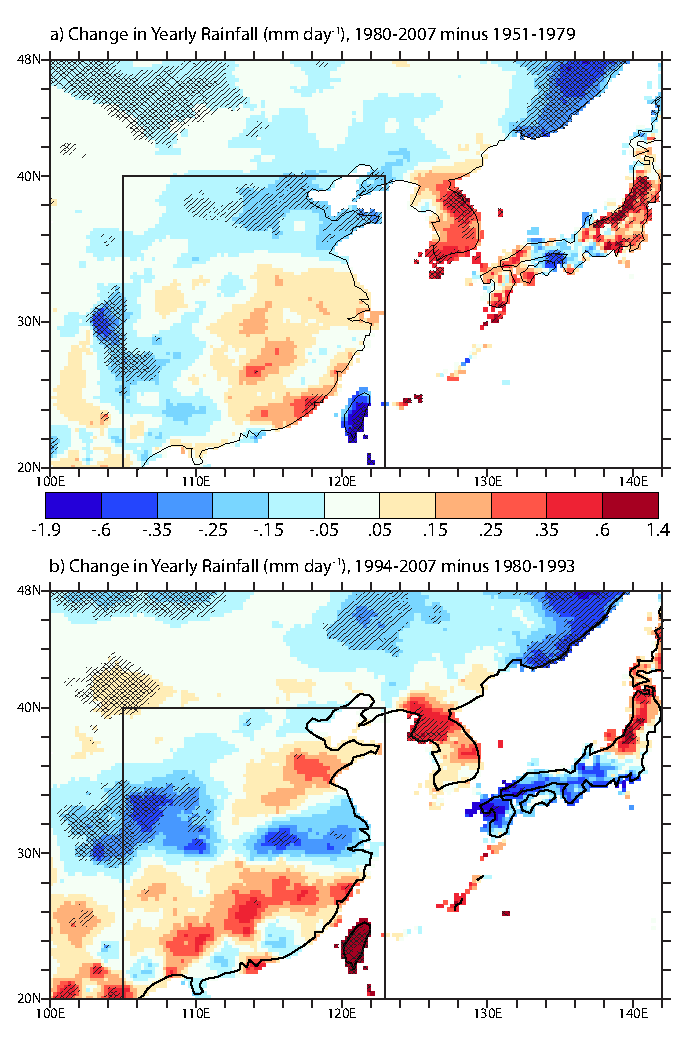
\includegraphics[width=32pc]{Figures/SFND}
\caption{Difference in East Asian yearly mean rainfall for a) 1980-2007 versus 1951-1979 and  b) 1994-2007 versus 1980-1993. The region of application of RDA spans 105-123$^{\circ}$E and 20-40$^{\circ}$N over eastern China and Taiwan (marked by box). Changes significant at a 95\%/99\% level are marked with single/double cross-hatches respectively as calculated by a bootstrap with replacement using 2,000 iterations.}
\label{fig:sfnd}
\end{figure}

\clearpage

\pnasbreak

\bibliography{RDA_SI_biblio}

\end{document}
